\documentclass[ignorenonframetext,]{beamer}
\setbeamertemplate{caption}[numbered]
\setbeamertemplate{caption label separator}{: }
\setbeamercolor{caption name}{fg=normal text.fg}
\beamertemplatenavigationsymbolsempty
\usepackage{lmodern}
\usepackage{amssymb,amsmath}
\usepackage{ifxetex,ifluatex}
\usepackage{fixltx2e} % provides \textsubscript
\ifnum 0\ifxetex 1\fi\ifluatex 1\fi=0 % if pdftex
  \usepackage[T1]{fontenc}
  \usepackage[utf8]{inputenc}
\else % if luatex or xelatex
  \ifxetex
    \usepackage{mathspec}
  \else
    \usepackage{fontspec}
  \fi
  \defaultfontfeatures{Ligatures=TeX,Scale=MatchLowercase}
\fi
% use upquote if available, for straight quotes in verbatim environments
\IfFileExists{upquote.sty}{\usepackage{upquote}}{}
% use microtype if available
\IfFileExists{microtype.sty}{%
\usepackage{microtype}
\UseMicrotypeSet[protrusion]{basicmath} % disable protrusion for tt fonts
}{}
\newif\ifbibliography
\hypersetup{
            pdftitle={Logistische Regression},
            pdfauthor={Prof.~Dr.~Karsten Lübke},
            pdfborder={0 0 0},
            breaklinks=true}
\urlstyle{same}  % don't use monospace font for urls
\usepackage{color}
\usepackage{fancyvrb}
\newcommand{\VerbBar}{|}
\newcommand{\VERB}{\Verb[commandchars=\\\{\}]}
\DefineVerbatimEnvironment{Highlighting}{Verbatim}{commandchars=\\\{\}}
% Add ',fontsize=\small' for more characters per line
\usepackage{framed}
\definecolor{shadecolor}{RGB}{248,248,248}
\newenvironment{Shaded}{\begin{snugshade}}{\end{snugshade}}
\newcommand{\KeywordTok}[1]{\textcolor[rgb]{0.13,0.29,0.53}{\textbf{{#1}}}}
\newcommand{\DataTypeTok}[1]{\textcolor[rgb]{0.13,0.29,0.53}{{#1}}}
\newcommand{\DecValTok}[1]{\textcolor[rgb]{0.00,0.00,0.81}{{#1}}}
\newcommand{\BaseNTok}[1]{\textcolor[rgb]{0.00,0.00,0.81}{{#1}}}
\newcommand{\FloatTok}[1]{\textcolor[rgb]{0.00,0.00,0.81}{{#1}}}
\newcommand{\ConstantTok}[1]{\textcolor[rgb]{0.00,0.00,0.00}{{#1}}}
\newcommand{\CharTok}[1]{\textcolor[rgb]{0.31,0.60,0.02}{{#1}}}
\newcommand{\SpecialCharTok}[1]{\textcolor[rgb]{0.00,0.00,0.00}{{#1}}}
\newcommand{\StringTok}[1]{\textcolor[rgb]{0.31,0.60,0.02}{{#1}}}
\newcommand{\VerbatimStringTok}[1]{\textcolor[rgb]{0.31,0.60,0.02}{{#1}}}
\newcommand{\SpecialStringTok}[1]{\textcolor[rgb]{0.31,0.60,0.02}{{#1}}}
\newcommand{\ImportTok}[1]{{#1}}
\newcommand{\CommentTok}[1]{\textcolor[rgb]{0.56,0.35,0.01}{\textit{{#1}}}}
\newcommand{\DocumentationTok}[1]{\textcolor[rgb]{0.56,0.35,0.01}{\textbf{\textit{{#1}}}}}
\newcommand{\AnnotationTok}[1]{\textcolor[rgb]{0.56,0.35,0.01}{\textbf{\textit{{#1}}}}}
\newcommand{\CommentVarTok}[1]{\textcolor[rgb]{0.56,0.35,0.01}{\textbf{\textit{{#1}}}}}
\newcommand{\OtherTok}[1]{\textcolor[rgb]{0.56,0.35,0.01}{{#1}}}
\newcommand{\FunctionTok}[1]{\textcolor[rgb]{0.00,0.00,0.00}{{#1}}}
\newcommand{\VariableTok}[1]{\textcolor[rgb]{0.00,0.00,0.00}{{#1}}}
\newcommand{\ControlFlowTok}[1]{\textcolor[rgb]{0.13,0.29,0.53}{\textbf{{#1}}}}
\newcommand{\OperatorTok}[1]{\textcolor[rgb]{0.81,0.36,0.00}{\textbf{{#1}}}}
\newcommand{\BuiltInTok}[1]{{#1}}
\newcommand{\ExtensionTok}[1]{{#1}}
\newcommand{\PreprocessorTok}[1]{\textcolor[rgb]{0.56,0.35,0.01}{\textit{{#1}}}}
\newcommand{\AttributeTok}[1]{\textcolor[rgb]{0.77,0.63,0.00}{{#1}}}
\newcommand{\RegionMarkerTok}[1]{{#1}}
\newcommand{\InformationTok}[1]{\textcolor[rgb]{0.56,0.35,0.01}{\textbf{\textit{{#1}}}}}
\newcommand{\WarningTok}[1]{\textcolor[rgb]{0.56,0.35,0.01}{\textbf{\textit{{#1}}}}}
\newcommand{\AlertTok}[1]{\textcolor[rgb]{0.94,0.16,0.16}{{#1}}}
\newcommand{\ErrorTok}[1]{\textcolor[rgb]{0.64,0.00,0.00}{\textbf{{#1}}}}
\newcommand{\NormalTok}[1]{{#1}}
\usepackage{longtable,booktabs}
\usepackage{caption}
% These lines are needed to make table captions work with longtable:
\makeatletter
\def\fnum@table{\tablename~\thetable}
\makeatother

% Prevent slide breaks in the middle of a paragraph:
\widowpenalties 1 10000
\raggedbottom

\AtBeginPart{
  \let\insertpartnumber\relax
  \let\partname\relax
  \frame{\partpage}
}
\AtBeginSection{
  \ifbibliography
  \else
    \let\insertsectionnumber\relax
    \let\sectionname\relax
    \frame{\sectionpage}
  \fi
}
\AtBeginSubsection{
  \let\insertsubsectionnumber\relax
  \let\subsectionname\relax
  \frame{\subsectionpage}
}

\setlength{\parindent}{0pt}
\setlength{\parskip}{6pt plus 2pt minus 1pt}
\setlength{\emergencystretch}{3em}  % prevent overfull lines
\providecommand{\tightlist}{%
  \setlength{\itemsep}{0pt}\setlength{\parskip}{0pt}}
\setcounter{secnumdepth}{0}
\usepackage[german]{babel}
\mode<presentation>
{
  \usetheme{fom}
  \useoutertheme{fomifes}
  \setbeamercovered{transparent}
}

\title{Logistische Regression}
\author{Prof.~Dr.~Karsten Lübke}
\date{SoSe 2017}

\begin{document}
\frame{\titlepage}

\begin{frame}{Modellierung}

\[y=f(x) + \epsilon \]

Hier nur für eine unabhängige Variable:

\begin{itemize}
\tightlist
\item
  Lineare Regression: abhängige Variable \(y\) numerisch:
  \(y_i=\beta_0 + \beta_1 \cdot x_i + \epsilon_i\)
\item
  Logistische Regression: abhängige Variable \(y\) binär, d. h.,
  kategorial mit zwei Merkmalsausprägungen \(y_i \in \{0,1\}\). \(p_i\)
  sei die Wahrscheinlichkeit, dass \(y_i=1\), dann:
  \(logit(p_i)=\ln(\frac{p_i}{1-p_i})=\beta_0 + \beta_1 \cdot x_i\)

  \begin{itemize}
  \tightlist
  \item
    Kunde/ kein Kunde
  \item
    Abwanderung Ja/ Nein
  \item
    Raucher/ Nichtraucher
  \item
    Kreditausfall Ja/ Nein
  \end{itemize}
\end{itemize}

\end{frame}

\begin{frame}{Analyse Extraversion}

Extraversionstest nach Dr.~Satow, angepasst von Prof.~Dr.~Sebastian
Sauer.

Fragebogen: \url{http://bit.ly/1HBhKWU}

\end{frame}

\begin{frame}[fragile]{Analyse Extraversionsdaten: Alternative Einlesen}

Menü RStudio:

\texttt{File\ -\textgreater{}\ Import\ Dataset-\textgreater{}\ From\ Excel\ ...}

Datei ``Extraversion.xlsx'' auswählen (\texttt{Browse})
\texttt{-\textgreater{}\ Import}

\end{frame}

\begin{frame}[fragile]{Analyse Extraversionsdaten: Einlesen}

\begin{Shaded}
\begin{Highlighting}[]
\CommentTok{# Gggfs. Einmalig vorab installieren}
\CommentTok{# install.packages("readxl")}

\CommentTok{# Paket zum Einlesen von Excel Dateien laden}
\KeywordTok{library}\NormalTok{(readxl)}

\CommentTok{# Daten einlesen}

\CommentTok{# Daten "Extraversion.xls" einlesen }
\CommentTok{# und als Datensatz "Extraversion" in R speichern}
\CommentTok{# Achtung: Pfad zur Datei anpassen}
\NormalTok{Extraversion <-}\StringTok{ }\KeywordTok{read_excel}\NormalTok{(}\StringTok{"Extraversion.xlsx"}\NormalTok{)}
\end{Highlighting}
\end{Shaded}

\end{frame}

\begin{frame}[fragile]{Bereitschaft sich freiwillig zur Messe zu melden}

Modellierung durch die Anzahl Facebook-Freunde.

\begin{Shaded}
\begin{Highlighting}[]
\KeywordTok{library}\NormalTok{(mosaic)}

\KeywordTok{xyplot}\NormalTok{( (F18_Messe==}\StringTok{"ja"}\NormalTok{) ~}\StringTok{ }\NormalTok{F12_Facebook, }
        \DataTypeTok{data =} \NormalTok{Extraversion)}
\end{Highlighting}
\end{Shaded}

\begin{center}\includegraphics[width=0.6\linewidth]{LogistischeRegression-Extraversion_files/figure-beamer/unnamed-chunk-1-1} \end{center}

\end{frame}

\begin{frame}{Modellierung Logit}

\[p(y=1)=\frac{e^\eta}{1+e^\eta}=\frac{e^{\beta_0 + \beta_1 \cdot x_i}}{1+e^{\beta_0 + \beta_1 \cdot x_i}} = \frac{1}{1+e^{-(\beta_0 + \beta_1 \cdot x_i)}}\]

\begin{center}\includegraphics[width=0.33\linewidth]{LogistischeRegression-Extraversion_files/figure-beamer/unnamed-chunk-2-1} \end{center}

Schätze \(\beta\) anhand der Daten: \(\hat{\beta}\):

\begin{itemize}
\tightlist
\item
  \(\beta>0\): Wahrscheinlichkeit steigt
\item
  \(\beta<0\): Wahrscheinlichkeit fällt
\end{itemize}

\end{frame}

\begin{frame}[fragile]{Vorbereitung: Modellierung Messebesuch}

R modelliert \(y\) anhand der \emph{Faktorstufen}: In der logistischen
Regression ist die erste Ausprägung die \(0\), alle weiteren \(1\)

\begin{Shaded}
\begin{Highlighting}[]
\CommentTok{# Als Faktor definieren}
\NormalTok{Extraversion$F18_Messe <-}\StringTok{ }\KeywordTok{factor}\NormalTok{(Extraversion$F18_Messe)}
\CommentTok{# Referenzklasse festelgen}
\NormalTok{Extraversion$F18_Messe <-}\StringTok{ }\KeywordTok{relevel}\NormalTok{(Extraversion$F18_Messe, }
                                  \DataTypeTok{ref=}\StringTok{"nein"}\NormalTok{)}
\CommentTok{# Kontrolle}
\KeywordTok{levels}\NormalTok{(Extraversion$F18_Messe)}
\end{Highlighting}
\end{Shaded}

\begin{verbatim}
## [1] "nein" "ja"
\end{verbatim}

\end{frame}

\begin{frame}[fragile]{Logistische Regression: Messebesuch}

\begin{Shaded}
\begin{Highlighting}[]
\NormalTok{ergglm <-}\StringTok{ }\KeywordTok{glm}\NormalTok{(F18_Messe ~}\StringTok{ }\NormalTok{F12_Facebook, }
              \DataTypeTok{data =} \NormalTok{Extraversion,}
              \DataTypeTok{family =} \KeywordTok{binomial}\NormalTok{(}\StringTok{"logit"}\NormalTok{))}
              
\KeywordTok{plotModel}\NormalTok{(ergglm)}
\end{Highlighting}
\end{Shaded}

\begin{center}\includegraphics[width=0.6\linewidth]{LogistischeRegression-Extraversion_files/figure-beamer/unnamed-chunk-4-1} \end{center}

\end{frame}

\begin{frame}[fragile]{Ergebnis Logistische Regression}

\begin{Shaded}
\begin{Highlighting}[]
\KeywordTok{summary}\NormalTok{(ergglm)}
\end{Highlighting}
\end{Shaded}

\begin{verbatim}
## 
## Call:
## glm(formula = F18_Messe ~ F12_Facebook, family = binomial("logit"), 
##     data = Extraversion)
## 
## Deviance Residuals: 
##    Min      1Q  Median      3Q     Max  
## -1.259  -1.071  -1.028   1.274   1.334  
## 
## Coefficients:
##                Estimate Std. Error z value Pr(>|z|)  
## (Intercept)  -0.3616264  0.1719854  -2.103   0.0355 *
## F12_Facebook  0.0004245  0.0004381   0.969   0.3326  
## ---
## Signif. codes:  0 '***' 0.001 '**' 0.01 '*' 0.05 '.' 0.1 ' ' 1
## 
## (Dispersion parameter for binomial family taken to be 1)
## 
##     Null deviance: 444.69  on 323  degrees of freedom
## Residual deviance: 443.75  on 322  degrees of freedom
## AIC: 447.75
## 
## Number of Fisher Scoring iterations: 4
\end{verbatim}

\end{frame}

\begin{frame}{Regressionskoeffizienten}

\begin{longtable}[]{@{}lrrrr@{}}
\toprule
\begin{minipage}[b]{0.19\columnwidth}\raggedright\strut
\strut
\end{minipage} & \begin{minipage}[b]{0.19\columnwidth}\raggedleft\strut
Estimate\strut
\end{minipage} & \begin{minipage}[b]{0.19\columnwidth}\raggedleft\strut
Std. Error\strut
\end{minipage} & \begin{minipage}[b]{0.19\columnwidth}\raggedleft\strut
z value\strut
\end{minipage} & \begin{minipage}[b]{0.19\columnwidth}\raggedleft\strut
Pr(\textgreater{}\textbar{}z\textbar{})\strut
\end{minipage}\tabularnewline
\midrule
\endhead
(Intercept) & -0.3616264 & 0.1719854 & -2.1026571 &
0.0354958\tabularnewline
F12\_Facebook & 0.0004245 & 0.0004381 & 0.9689802 &
0.3325550\tabularnewline
\bottomrule
\end{longtable}

\end{frame}

\begin{frame}{Übung 1: Regressionskoeffizienten}

Welche der folgenden Aussagen stimmt?

\begin{itemize}
\tightlist
\item
  A: In der Stichprobe steigt die Bereitschaft sich freiwillig zur Messe
  zu melden mit der Anzahl der Facebook-Freunde
\item
  B: In der Stichprobe sinkt die Bereitschaft sich freiwillig zur Messe
  zu melden mit der Anzahl der Facebook-Freunde
\item
  C: In der Stichprobe ist die Bereitschaft sich freiwillig zur Messe zu
  melden unverändert mit der Anzahl der Facebook-Freunde
\end{itemize}

\end{frame}

\begin{frame}[fragile]{Bootstrap Regressionkoeffizient (I/II)}

\begin{Shaded}
\begin{Highlighting}[]
\KeywordTok{set.seed}\NormalTok{(}\DecValTok{1896}\NormalTok{)}

\NormalTok{Bootvtlg <-}\StringTok{ }\KeywordTok{do}\NormalTok{(}\DecValTok{5000}\NormalTok{) *}
\StringTok{  }\KeywordTok{coef}\NormalTok{(}\KeywordTok{glm}\NormalTok{(F18_Messe ~}\StringTok{ }\NormalTok{F12_Facebook, }
           \DataTypeTok{data =} \KeywordTok{resample}\NormalTok{(Extraversion),}
           \DataTypeTok{family =} \KeywordTok{binomial}\NormalTok{(}\StringTok{"logit"}\NormalTok{)))[}\DecValTok{2}\NormalTok{]}
\end{Highlighting}
\end{Shaded}

\end{frame}

\begin{frame}[fragile]{Bootstrap Regressionkoeffizient (II/II)}

\begin{Shaded}
\begin{Highlighting}[]
\KeywordTok{histogram}\NormalTok{( ~}\StringTok{ }\NormalTok{F12_Facebook, }\DataTypeTok{data =} \NormalTok{Bootvtlg)}
\end{Highlighting}
\end{Shaded}

\begin{center}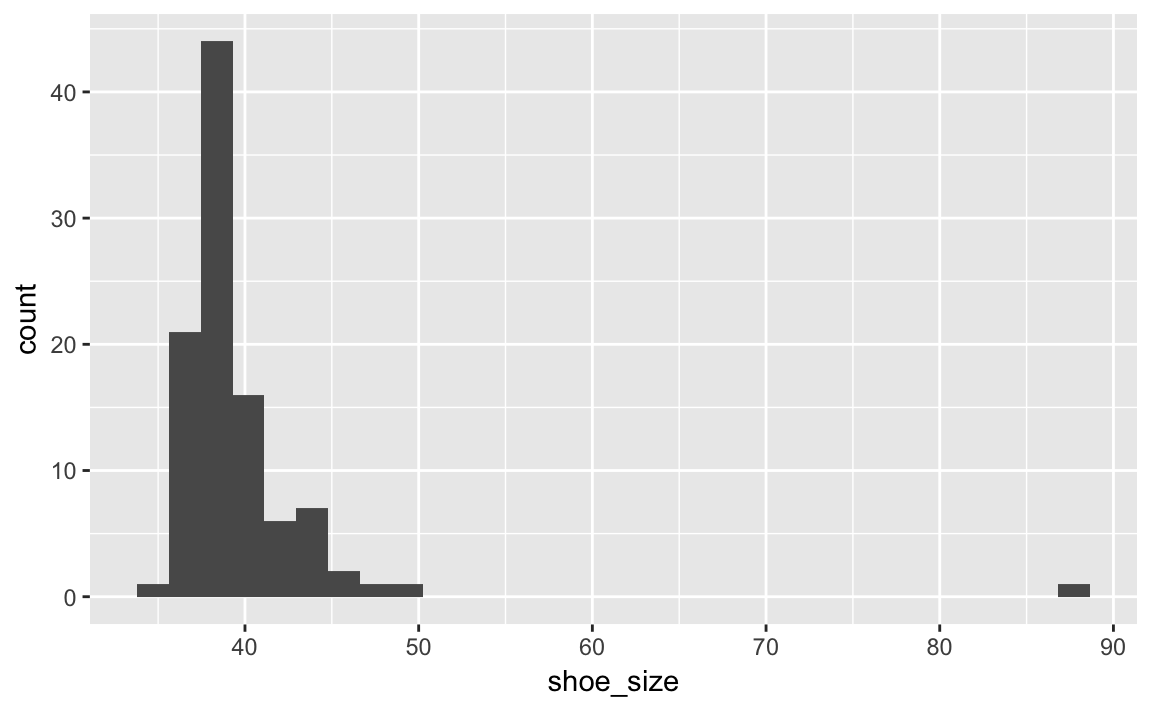
\includegraphics[width=0.4\linewidth]{LogistischeRegression-Extraversion_files/figure-beamer/unnamed-chunk-8-1} \end{center}

\begin{Shaded}
\begin{Highlighting}[]
\KeywordTok{quantile}\NormalTok{( ~}\StringTok{ }\NormalTok{F12_Facebook, }\DataTypeTok{data =} \NormalTok{Bootvtlg, }
          \DataTypeTok{probs =} \KeywordTok{c}\NormalTok{(}\FloatTok{0.025}\NormalTok{, }\FloatTok{0.975}\NormalTok{))}
\end{Highlighting}
\end{Shaded}

\begin{verbatim}
##          2.5%         97.5% 
## -0.0004170976  0.0013528616
\end{verbatim}

\end{frame}

\begin{frame}{Übung 2: Inferenz: Nullhypothese}

Wie lautet die Nullhypothese, wenn die Variable \(x\) keinen Einfluss
auf \(p(y=1)\) in der Population hat:

\begin{itemize}
\tightlist
\item
  A: \(H_0: \beta_1=0\)
\item
  B: \(H_0: \beta_1=1\)
\item
  C: \(H_0: \hat{\beta}_1=0\)
\item
  D: \(H_0: \hat{\beta}_1=1\)
\end{itemize}

\end{frame}

\begin{frame}[fragile]{Permutationstest Regressionskoeffizient (I/II)}

\begin{Shaded}
\begin{Highlighting}[]
\NormalTok{Nullvtlg <-}\StringTok{ }\KeywordTok{do}\NormalTok{(}\DecValTok{5000}\NormalTok{) *}
\StringTok{  }\KeywordTok{coef}\NormalTok{(}\KeywordTok{glm}\NormalTok{(F18_Messe ~}\StringTok{ }\KeywordTok{shuffle}\NormalTok{(F12_Facebook), }
           \DataTypeTok{data =} \NormalTok{Extraversion,}
           \DataTypeTok{family =} \KeywordTok{binomial}\NormalTok{(}\StringTok{"logit"}\NormalTok{)))[}\DecValTok{2}\NormalTok{]}
\end{Highlighting}
\end{Shaded}

\end{frame}

\begin{frame}[fragile]{Permutationstest Regressionskoeffizient (II/II)}

\begin{Shaded}
\begin{Highlighting}[]
\KeywordTok{histogram}\NormalTok{( ~}\StringTok{ }\NormalTok{F12_Facebook, }\DataTypeTok{data =} \NormalTok{Nullvtlg)}
\end{Highlighting}
\end{Shaded}

\begin{center}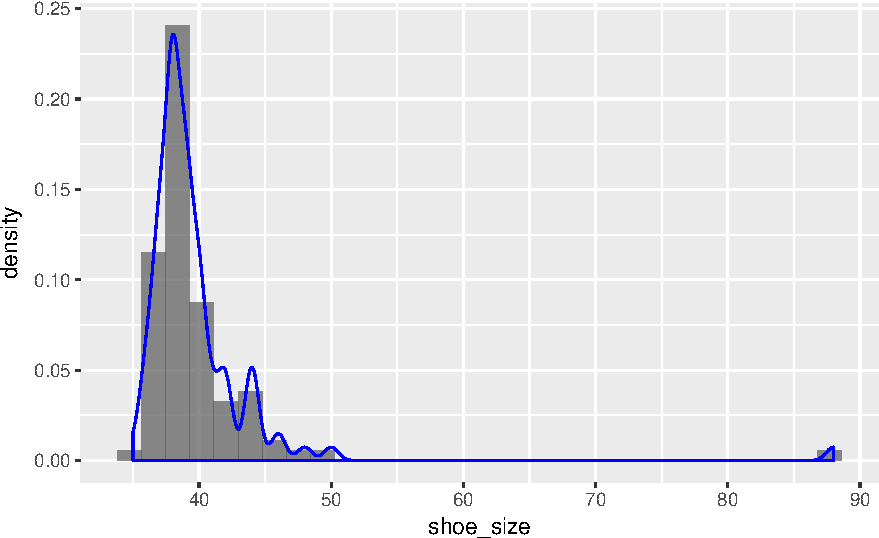
\includegraphics[width=0.33\linewidth]{LogistischeRegression-Extraversion_files/figure-beamer/unnamed-chunk-10-1} \end{center}

\begin{Shaded}
\begin{Highlighting}[]
\KeywordTok{prop}\NormalTok{( ~}\StringTok{ }\KeywordTok{abs}\NormalTok{(F12_Facebook) >=}\StringTok{ }\KeywordTok{coef}\NormalTok{(ergglm)[}\DecValTok{2}\NormalTok{], }
      \DataTypeTok{data=}\NormalTok{Nullvtlg )}
\end{Highlighting}
\end{Shaded}

\begin{verbatim}
##   TRUE 
## 0.3298
\end{verbatim}

\end{frame}

\begin{frame}{Übung 3: Inferenz Anzahl Facebook Freunde}

Liefern die Daten Belege dafür, einen Zusammenhang zwischen der Anzahl
Facebook-Freunde und der Bereitschaft sich freiwillig zur Messe zu
melden in der Population zu zeigen (Forschungsthese)?

\begin{itemize}
\tightlist
\item
  Ja.
\item
  Nein.
\end{itemize}

\end{frame}

\begin{frame}[fragile]{Modellierung Messebesuch durch Alter}

\begin{Shaded}
\begin{Highlighting}[]
\NormalTok{ergglm2 <-}\StringTok{ }\KeywordTok{glm}\NormalTok{(F18_Messe ~}\StringTok{ }\NormalTok{F14_Alter, }
              \DataTypeTok{data =} \NormalTok{Extraversion,}
              \DataTypeTok{family =} \KeywordTok{binomial}\NormalTok{(}\StringTok{"logit"}\NormalTok{))}
              
\KeywordTok{summary}\NormalTok{(ergglm2)}
\end{Highlighting}
\end{Shaded}

\begin{verbatim}
## 
## Call:
## glm(formula = F18_Messe ~ F14_Alter, family = binomial("logit"), 
##     data = Extraversion)
## 
## Deviance Residuals: 
##    Min      1Q  Median      3Q     Max  
## -1.199  -1.071  -1.035   1.278   1.336  
## 
## Coefficients:
##             Estimate Std. Error z value Pr(>|z|)
## (Intercept) -0.78278    0.67527  -1.159    0.246
## F14_Alter    0.02195    0.02669   0.822    0.411
## 
## (Dispersion parameter for binomial family taken to be 1)
## 
##     Null deviance: 444.69  on 323  degrees of freedom
## Residual deviance: 444.02  on 322  degrees of freedom
## AIC: 448.02
## 
## Number of Fisher Scoring iterations: 4
\end{verbatim}

\end{frame}

\begin{frame}{Koeffizienten Modellierung Messebesuch durch Alter}

\begin{longtable}[]{@{}lrrrr@{}}
\toprule
\begin{minipage}[b]{0.19\columnwidth}\raggedright\strut
\strut
\end{minipage} & \begin{minipage}[b]{0.19\columnwidth}\raggedleft\strut
Estimate\strut
\end{minipage} & \begin{minipage}[b]{0.19\columnwidth}\raggedleft\strut
Std. Error\strut
\end{minipage} & \begin{minipage}[b]{0.19\columnwidth}\raggedleft\strut
z value\strut
\end{minipage} & \begin{minipage}[b]{0.19\columnwidth}\raggedleft\strut
Pr(\textgreater{}\textbar{}z\textbar{})\strut
\end{minipage}\tabularnewline
\midrule
\endhead
(Intercept) & -0.7827803 & 0.6752712 & -1.1592087 &
0.2463711\tabularnewline
F14\_Alter & 0.0219464 & 0.0266934 & 0.8221656 &
0.4109826\tabularnewline
\bottomrule
\end{longtable}

\end{frame}

\begin{frame}{Übung 4: Ergebnis Modellierung Messebesuch durch Alter}

Wer hat im Modell die höchste Wahrscheinlichkeit sich freiwillig zur
Messe zu melden?

\begin{itemize}
\tightlist
\item
  A: Max, 20 Jahre
\item
  B: Tina, 24 Jahre
\item
  C: Susi, 30 Jahre
\end{itemize}

\end{frame}

\begin{frame}[fragile]{Übung 5: Inferenz Modellierung Messebesuch durch
Alter}

Ist in dem Modell der Einfluss der Variable \texttt{F14\_Alter}
\emph{signifikant}?

\begin{itemize}
\tightlist
\item
  Ja.
\item
  Nein.
\end{itemize}

\end{frame}

\begin{frame}[fragile]{Vorhersagen Logistische Regression}

Für Susi, 30 Jahre:

\begin{Shaded}
\begin{Highlighting}[]
\KeywordTok{predict}\NormalTok{(ergglm2, }
        \DataTypeTok{newdata =} \KeywordTok{data.frame}\NormalTok{(}\DataTypeTok{F14_Alter=}\DecValTok{30}\NormalTok{), }
        \DataTypeTok{type=}\StringTok{"response"}\NormalTok{)}
\end{Highlighting}
\end{Shaded}

\begin{verbatim}
##         1 
## 0.4689432
\end{verbatim}

\end{frame}

\begin{frame}[fragile]{Modellierung Messebesuch durch Geschlecht}

\begin{Shaded}
\begin{Highlighting}[]
\NormalTok{ergglm3 <-}\StringTok{ }\KeywordTok{glm}\NormalTok{(F18_Messe ~}\StringTok{ }\NormalTok{F15_Geschlecht, }
              \DataTypeTok{data =} \NormalTok{Extraversion,}
              \DataTypeTok{family =} \KeywordTok{binomial}\NormalTok{(}\StringTok{"logit"}\NormalTok{))}
              
\KeywordTok{summary}\NormalTok{(ergglm3)}
\end{Highlighting}
\end{Shaded}

\begin{verbatim}
## 
## Call:
## glm(formula = F18_Messe ~ F15_Geschlecht, family = binomial("logit"), 
##     data = Extraversion)
## 
## Deviance Residuals: 
##     Min       1Q   Median       3Q      Max  
## -1.2392  -0.9809  -0.9809   1.1168   1.3875  
## 
## Coefficients:
##                    Estimate Std. Error z value Pr(>|z|)    
## (Intercept)         -0.4815     0.1459  -3.300 0.000968 ***
## F15_GeschlechtMann   0.6257     0.2312   2.706 0.006804 ** 
## ---
## Signif. codes:  0 '***' 0.001 '**' 0.01 '*' 0.05 '.' 0.1 ' ' 1
## 
## (Dispersion parameter for binomial family taken to be 1)
## 
##     Null deviance: 444.69  on 323  degrees of freedom
## Residual deviance: 437.30  on 322  degrees of freedom
## AIC: 441.3
## 
## Number of Fisher Scoring iterations: 4
\end{verbatim}

\end{frame}

\begin{frame}{Koeffizienten Modellierung Messebesuch durch Geschlecht}

\begin{longtable}[]{@{}lrrrr@{}}
\toprule
\begin{minipage}[b]{0.19\columnwidth}\raggedright\strut
\strut
\end{minipage} & \begin{minipage}[b]{0.19\columnwidth}\raggedleft\strut
Estimate\strut
\end{minipage} & \begin{minipage}[b]{0.19\columnwidth}\raggedleft\strut
Std. Error\strut
\end{minipage} & \begin{minipage}[b]{0.19\columnwidth}\raggedleft\strut
z value\strut
\end{minipage} & \begin{minipage}[b]{0.19\columnwidth}\raggedleft\strut
Pr(\textgreater{}\textbar{}z\textbar{})\strut
\end{minipage}\tabularnewline
\midrule
\endhead
(Intercept) & -0.4814510 & 0.1459040 & -3.299780 &
0.0009676\tabularnewline
F15\_GeschlechtMann & 0.6257006 & 0.2312028 & 2.706285 &
0.0068041\tabularnewline
\bottomrule
\end{longtable}

\end{frame}

\begin{frame}{Übung 6: Ergebnis Modellierung Messebesuch durch
Geschlecht}

Wer hat im Modell die höchste Wahrscheinlichkeit sich freiwillig zur
Messe zu melden?

\begin{itemize}
\tightlist
\item
  A: Max
\item
  B: Tina
\item
  C: Beide gleich
\end{itemize}

\end{frame}

\begin{frame}{Übung 7: Inferenz Modellierung Messebesuch durch
Geschlecht}

Kann im Modell die Nullhypothese \(\beta_{\text{F15\_Geschlecht}}=0\)
verworfen werden?

\begin{itemize}
\tightlist
\item
  Ja.
\item
  Nein.
\end{itemize}

\end{frame}

\begin{frame}[fragile]{Odds Ratio}

\[OR=\frac{\frac{p_{\text{Mann}}}{1-p_{\text{Mann}}}}{\frac{p_{\text{Frau}}}{1-p_{\text{Frau}}}}\]

\begin{Shaded}
\begin{Highlighting}[]
\KeywordTok{exp}\NormalTok{(}\KeywordTok{coef}\NormalTok{(ergglm3))}
\end{Highlighting}
\end{Shaded}

\begin{verbatim}
##        (Intercept) F15_GeschlechtMann 
##          0.6178862          1.8695554
\end{verbatim}

Die Chance, dass sich ein Mann freiwillig meldet ist 1.87 mal so groß
wie die einer Frau.

\end{frame}

\begin{frame}[fragile]{Multiple Logistische Regression}

\begin{Shaded}
\begin{Highlighting}[]
\NormalTok{ergglm4 <-}\StringTok{ }\KeywordTok{glm}\NormalTok{(F18_Messe ~}\StringTok{ }\NormalTok{F14_Alter }
               \NormalTok{+}\StringTok{ }\NormalTok{F15_Geschlecht}
               \NormalTok{+}\StringTok{ }\NormalTok{F12_Facebook,}
              \DataTypeTok{data =} \NormalTok{Extraversion,}
              \DataTypeTok{family =} \KeywordTok{binomial}\NormalTok{(}\StringTok{"logit"}\NormalTok{))}
              
\KeywordTok{summary}\NormalTok{(ergglm4)}
\end{Highlighting}
\end{Shaded}

\begin{verbatim}
## 
## Call:
## glm(formula = F18_Messe ~ F14_Alter + F15_Geschlecht + F12_Facebook, 
##     family = binomial("logit"), data = Extraversion)
## 
## Deviance Residuals: 
##     Min       1Q   Median       3Q      Max  
## -1.3645  -1.0245  -0.9356   1.1868   1.4687  
## 
## Coefficients:
##                      Estimate Std. Error z value Pr(>|z|)  
## (Intercept)        -1.1901749  0.7730309  -1.540    0.124  
## F14_Alter           0.0234367  0.0287012   0.817    0.414  
## F15_GeschlechtMann  0.5879846  0.2340288   2.512    0.012 *
## F12_Facebook        0.0004693  0.0004675   1.004    0.315  
## ---
## Signif. codes:  0 '***' 0.001 '**' 0.01 '*' 0.05 '.' 0.1 ' ' 1
## 
## (Dispersion parameter for binomial family taken to be 1)
## 
##     Null deviance: 444.69  on 323  degrees of freedom
## Residual deviance: 436.02  on 320  degrees of freedom
## AIC: 444.02
## 
## Number of Fisher Scoring iterations: 4
\end{verbatim}

\end{frame}

\begin{frame}{Koeffizienten Multiple Logistische Regression}

\begin{longtable}[]{@{}lrrrr@{}}
\toprule
\begin{minipage}[b]{0.19\columnwidth}\raggedright\strut
\strut
\end{minipage} & \begin{minipage}[b]{0.19\columnwidth}\raggedleft\strut
Estimate\strut
\end{minipage} & \begin{minipage}[b]{0.19\columnwidth}\raggedleft\strut
Std. Error\strut
\end{minipage} & \begin{minipage}[b]{0.19\columnwidth}\raggedleft\strut
z value\strut
\end{minipage} & \begin{minipage}[b]{0.19\columnwidth}\raggedleft\strut
Pr(\textgreater{}\textbar{}z\textbar{})\strut
\end{minipage}\tabularnewline
\midrule
\endhead
(Intercept) & -1.1901749 & 0.7730309 & -1.5396214 &
0.1236527\tabularnewline
F14\_Alter & 0.0234367 & 0.0287012 & 0.8165753 &
0.4141712\tabularnewline
F15\_GeschlechtMann & 0.5879846 & 0.2340288 & 2.5124453 &
0.0119898\tabularnewline
F12\_Facebook & 0.0004693 & 0.0004675 & 1.0040207 &
0.3153686\tabularnewline
\bottomrule
\end{longtable}

\end{frame}

\begin{frame}{Übung 8: Ergebnis Multiple Logistische Regression}

Welche Variablen erhöhen die Wahrscheinlichkeit im Modell, dass sich die
Person freiwillig zur Messe meldet?

\begin{itemize}
\tightlist
\item
  A: Nur steigendes Alter
\item
  B: Nur Geschlecht Mann
\item
  C: Nur steigende Anzahl Facebook-Freunde
\item
  D: Alle Variablen
\item
  E: Keine der Variablen
\end{itemize}

\end{frame}

\begin{frame}{Übung 9: Inferenz Multiple Logistische Regression}

Welche Variablen sind \emph{signifikant}?

\begin{itemize}
\tightlist
\item
  A: Nur Alter
\item
  B: Nur Geschlecht
\item
  C: Nur Anzahl Facebook-Freunde
\item
  D: Alle Variablen
\item
  E: Keine der Variablen
\end{itemize}

\end{frame}

\begin{frame}[fragile]{Offene Übung: Modellierung Geschlecht}

Modellieren Sie die Wahrscheinlichkeit, dass es sich bei einer Person um
eine Frau handelt als Funktion der Variablen \texttt{F12\_Facebook},
\texttt{F13\_Kater}, \texttt{F19\_Partybesuche}.

\end{frame}

\end{document}
